%!TEX root = ../../../../report.tex
\subsection{Computer-Aided Design (CAD)} % (fold)
\label{sub:computer_aided_design}
Based on the defined boundaries of the previous sections, the necessary parts have been designed.
The modeling has been design-oriented manufacturing having in mind the 3D printing technology where not all kind of geometries can be printed with the same resolution and quality.

Generally, the parts have followed a round design avoiding cutting edges except where completely necessary.
Some corrections have been applied to the tolerances of the internal holes as explained in the section \ref{sub:arc_compensation}.
The implementation of the CAD design can be considered partially parametric due to, for its construction, a file with some parameters is used in several parts of the design.
This works so in the reconstruction of the part the program reads the file and change everything according to its parameters.
The used values are shown in the appendix \ref{app:cad_parameters}.
The results can be seen in the figures from \ref{fig:left_foot} to \ref{fig:knee_upper}.

\begin{figure}[ht!]
    \centering
    \begin{subfigure}[b]{0.49\textwidth}
        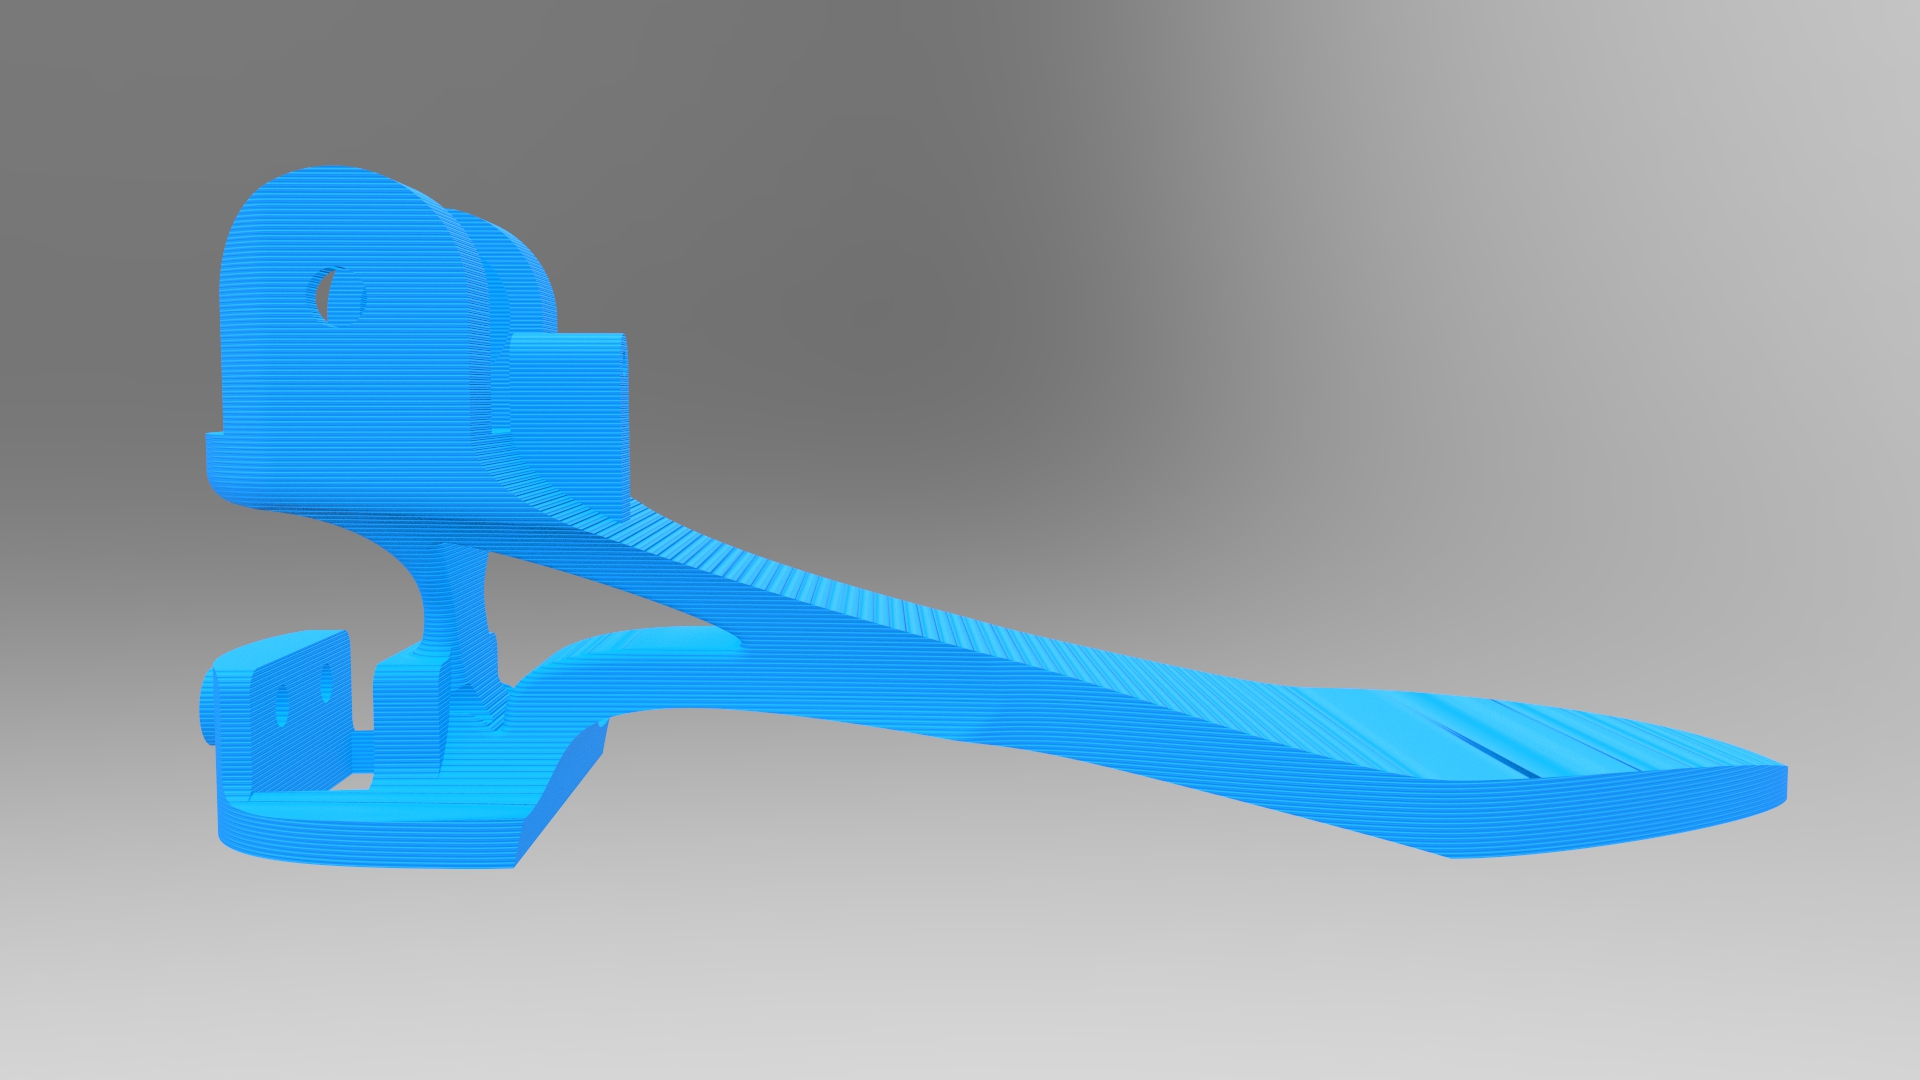
\includegraphics[width=\textwidth]{figures/legs_foot.jpg}
        \caption{Left foot}
        \label{fig:left_foot}
    \end{subfigure}
    \begin{subfigure}[b]{0.49\textwidth}
        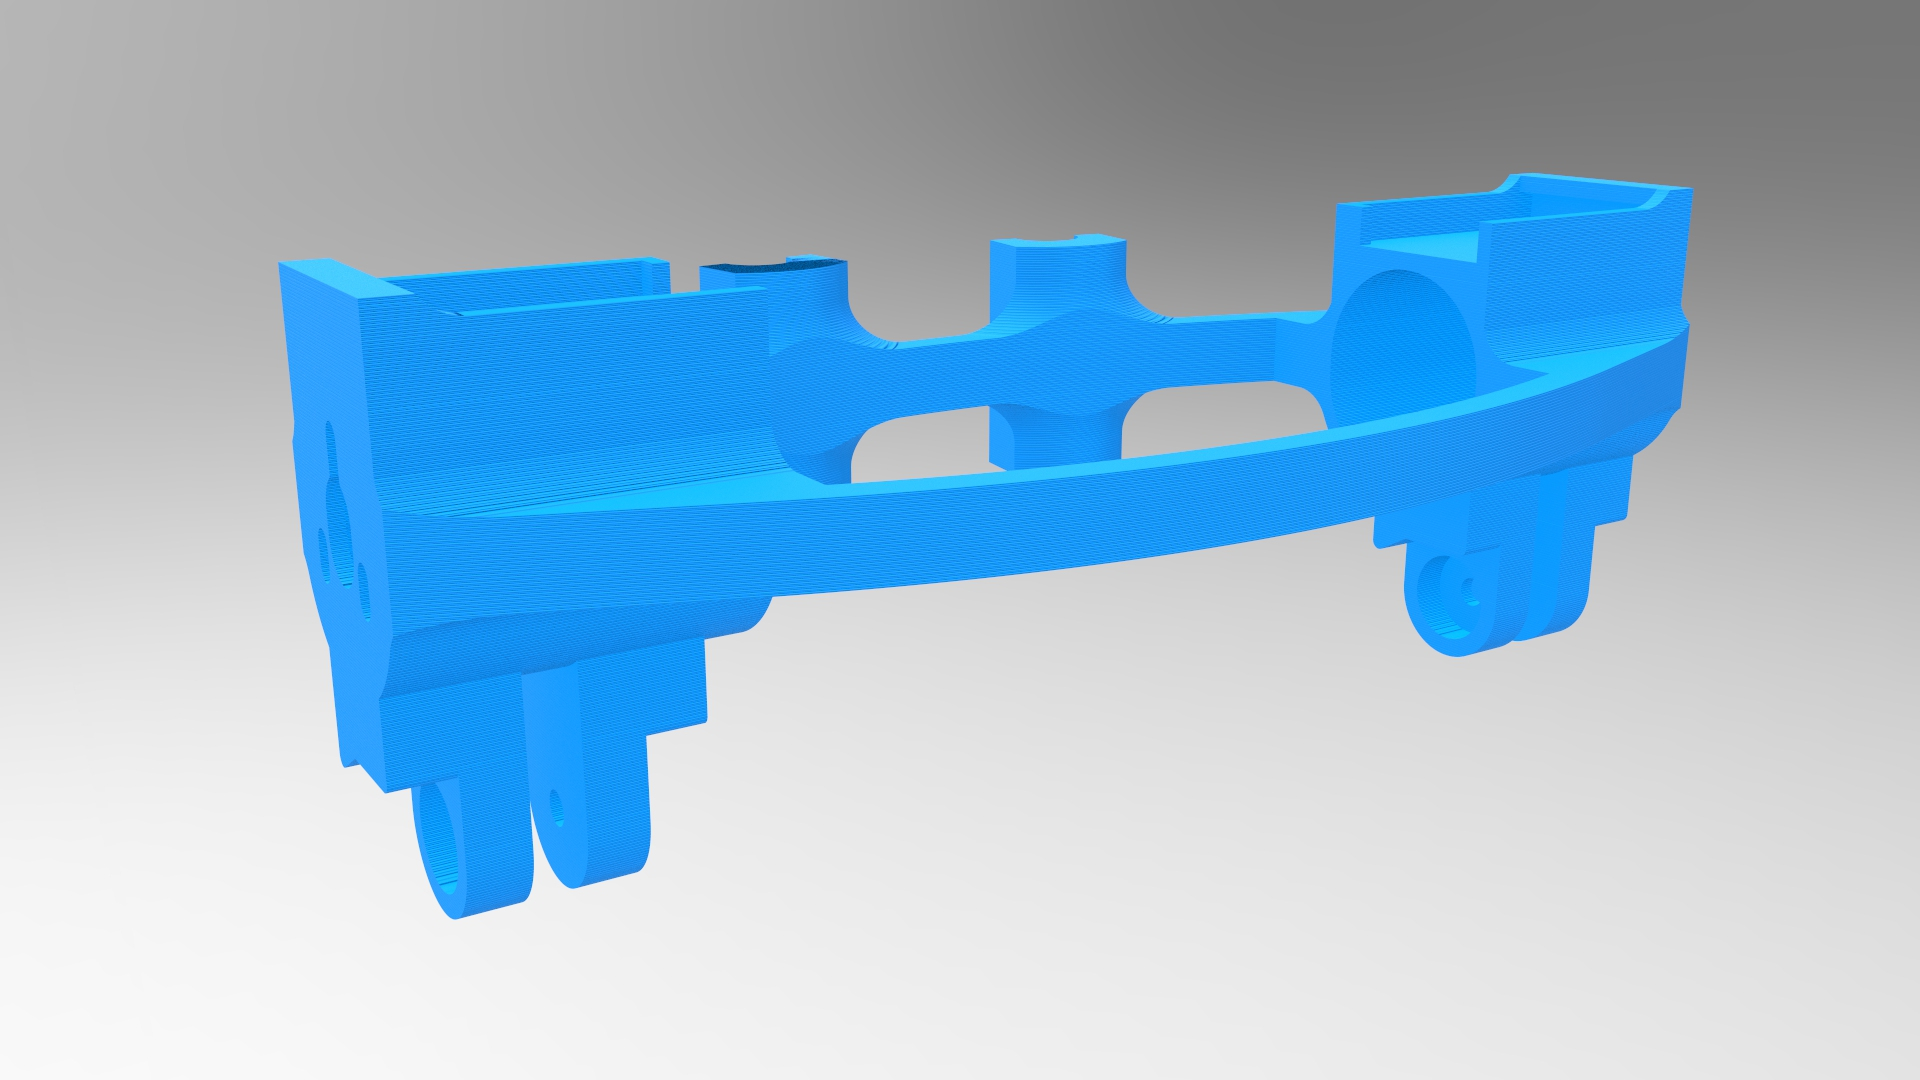
\includegraphics[width=\textwidth]{figures/legs_hip.jpg}
        \caption{Hip}
        \label{fig:hip}
    \end{subfigure}
\end{figure}    

\begin{figure}[ht!]
    \ContinuedFloat % continue from previous page
    \begin{subfigure}[b]{0.49\textwidth}
        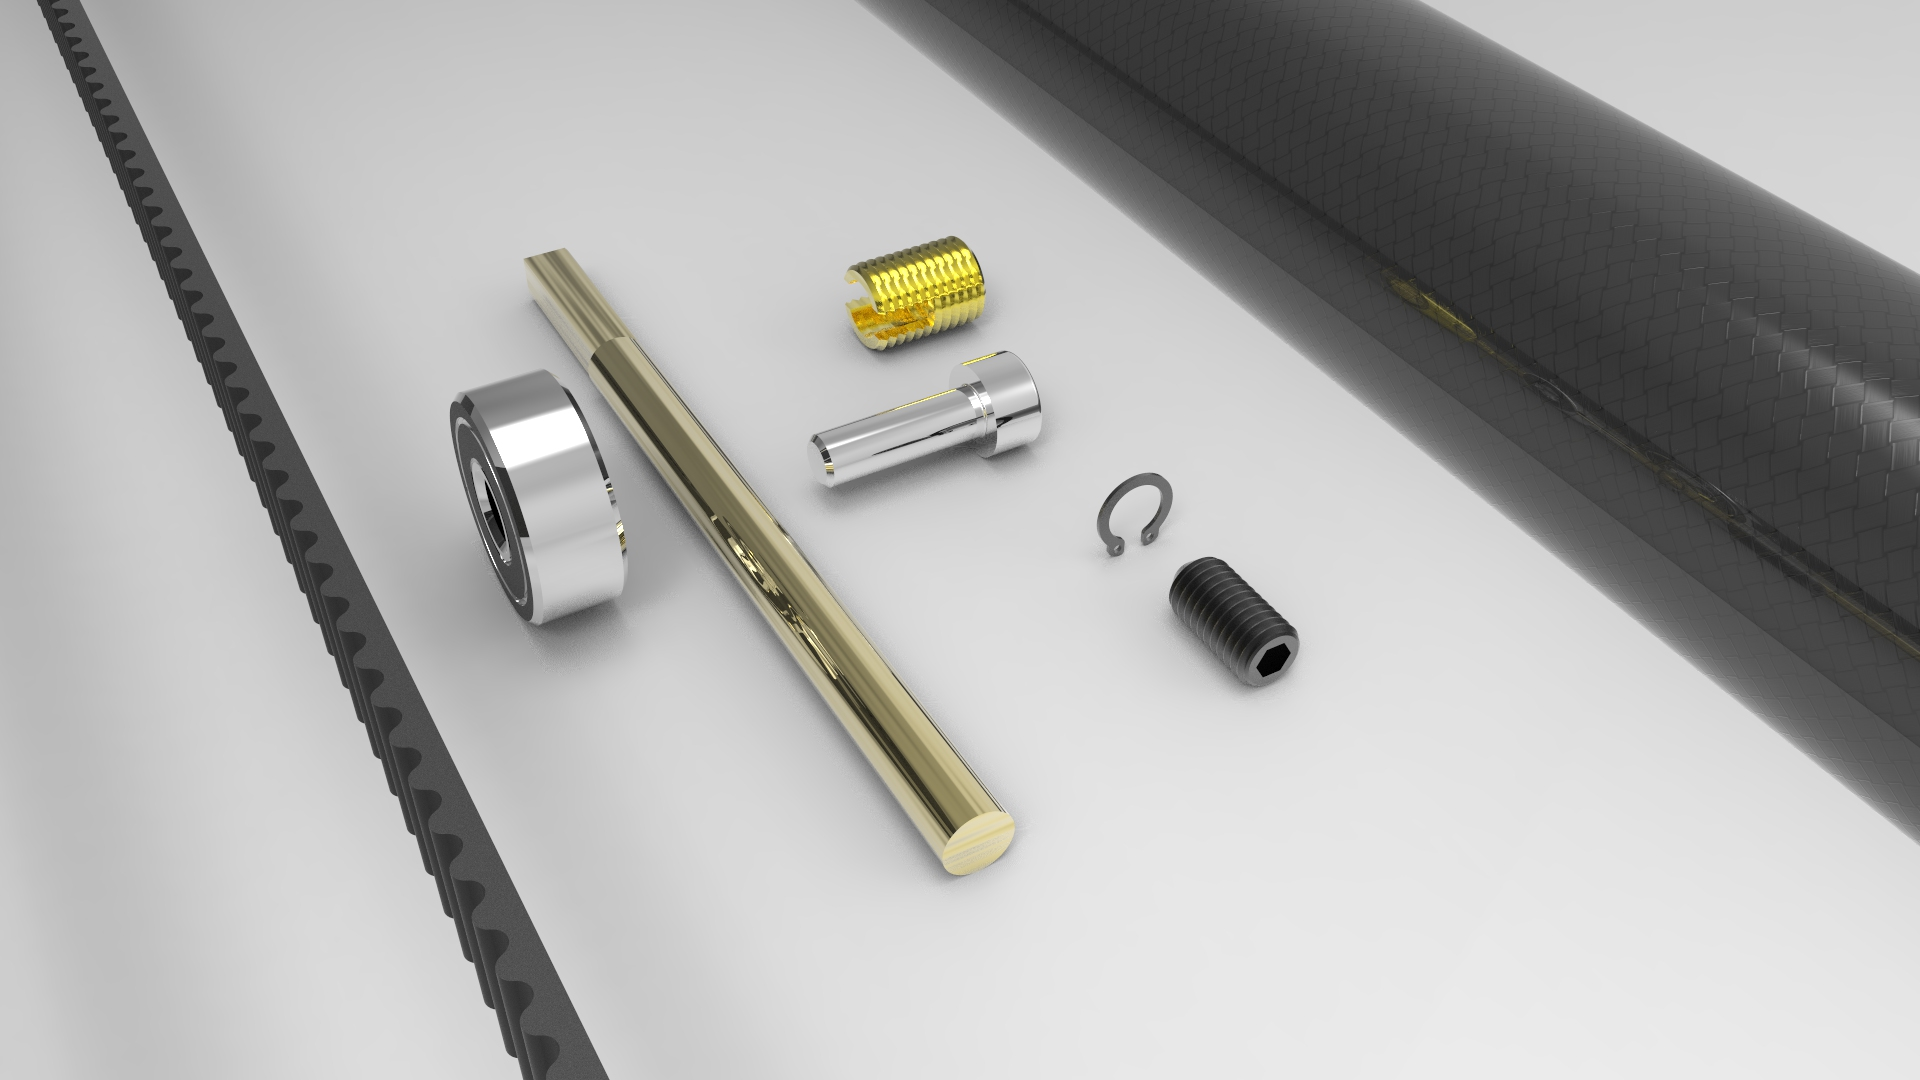
\includegraphics[width=\textwidth]{figures/legs_parts.jpg}
        \caption{Additional designed parts}
        \label{fig:mouse}
    \end{subfigure}
    \begin{subfigure}[b]{0.49\textwidth}
        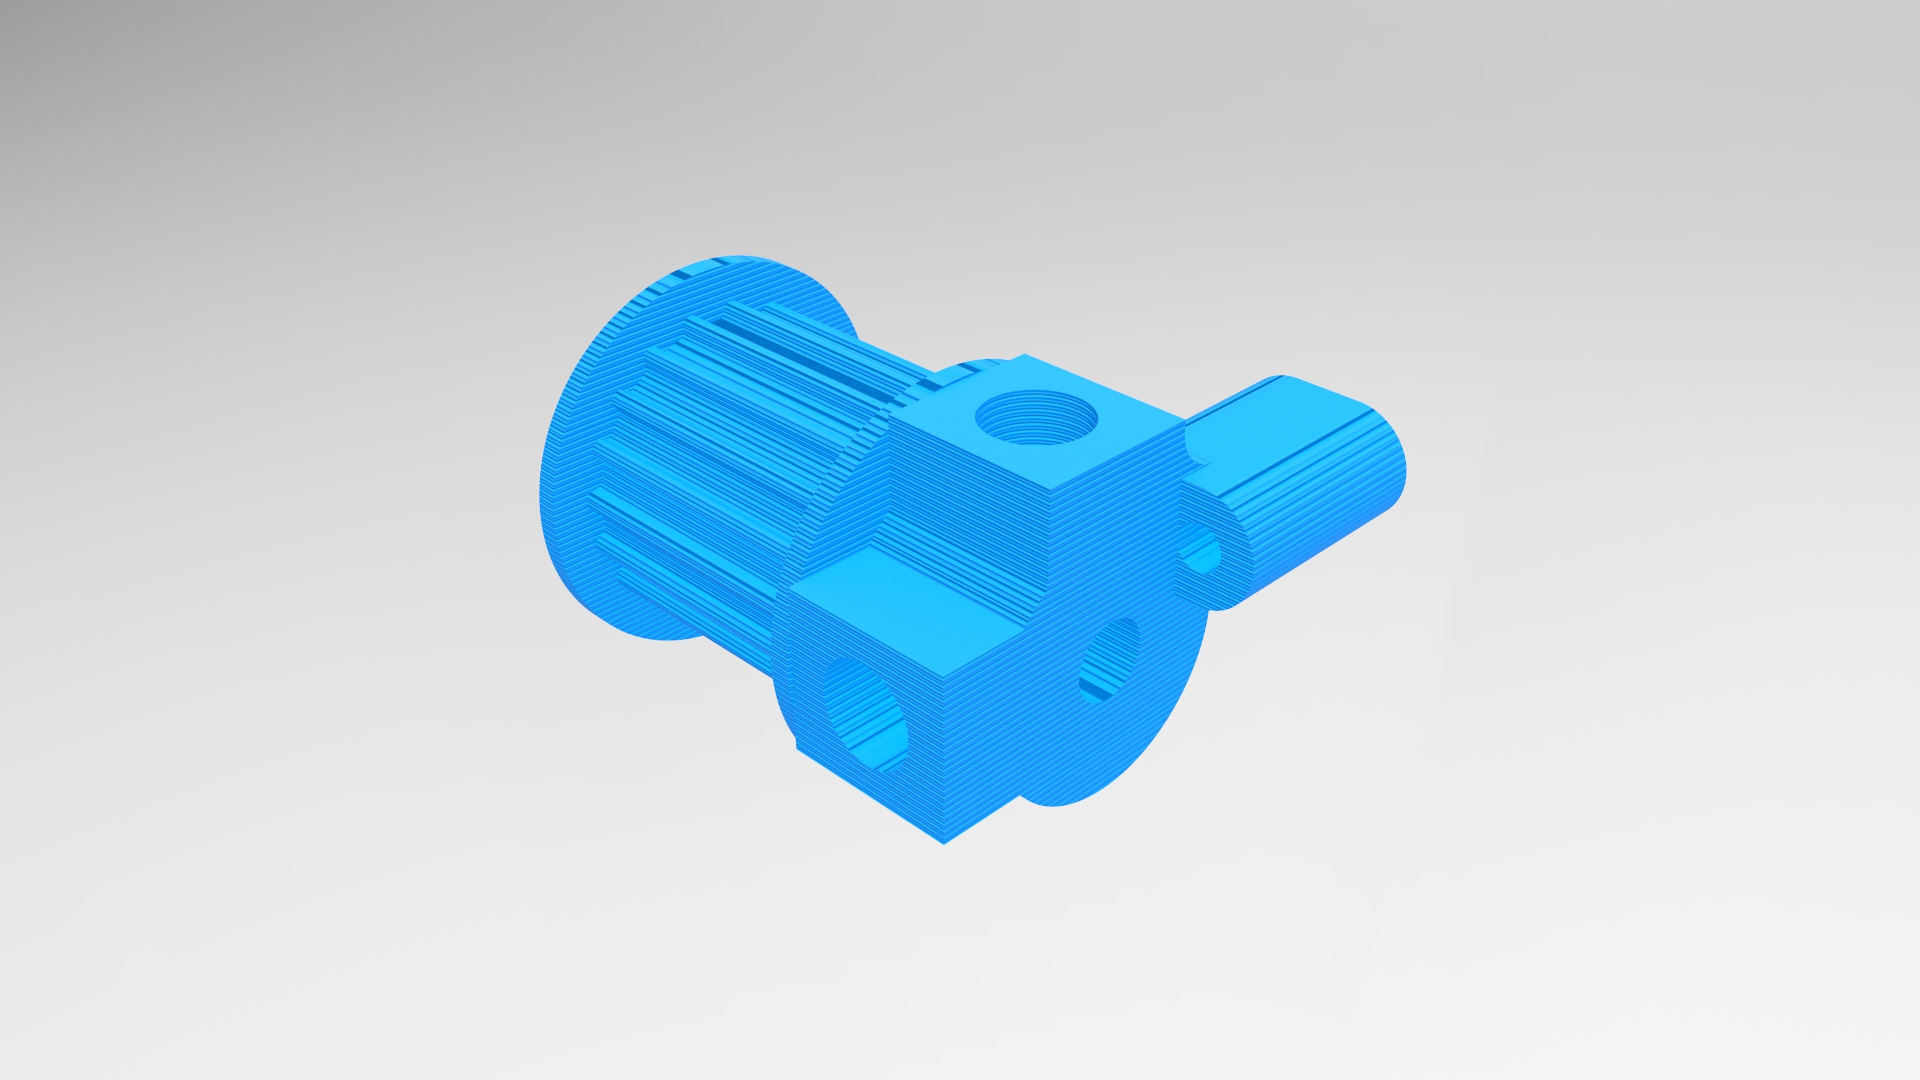
\includegraphics[width=\textwidth]{figures/legs_pulley.jpg}
        \caption{Left ankle serial spring pulley}
        \label{fig:serial_spring_pulley}
    \end{subfigure}
\end{figure}    

\begin{figure}[ht!]
    \ContinuedFloat % continue from previous page
    \begin{subfigure}[b]{0.49\textwidth}
        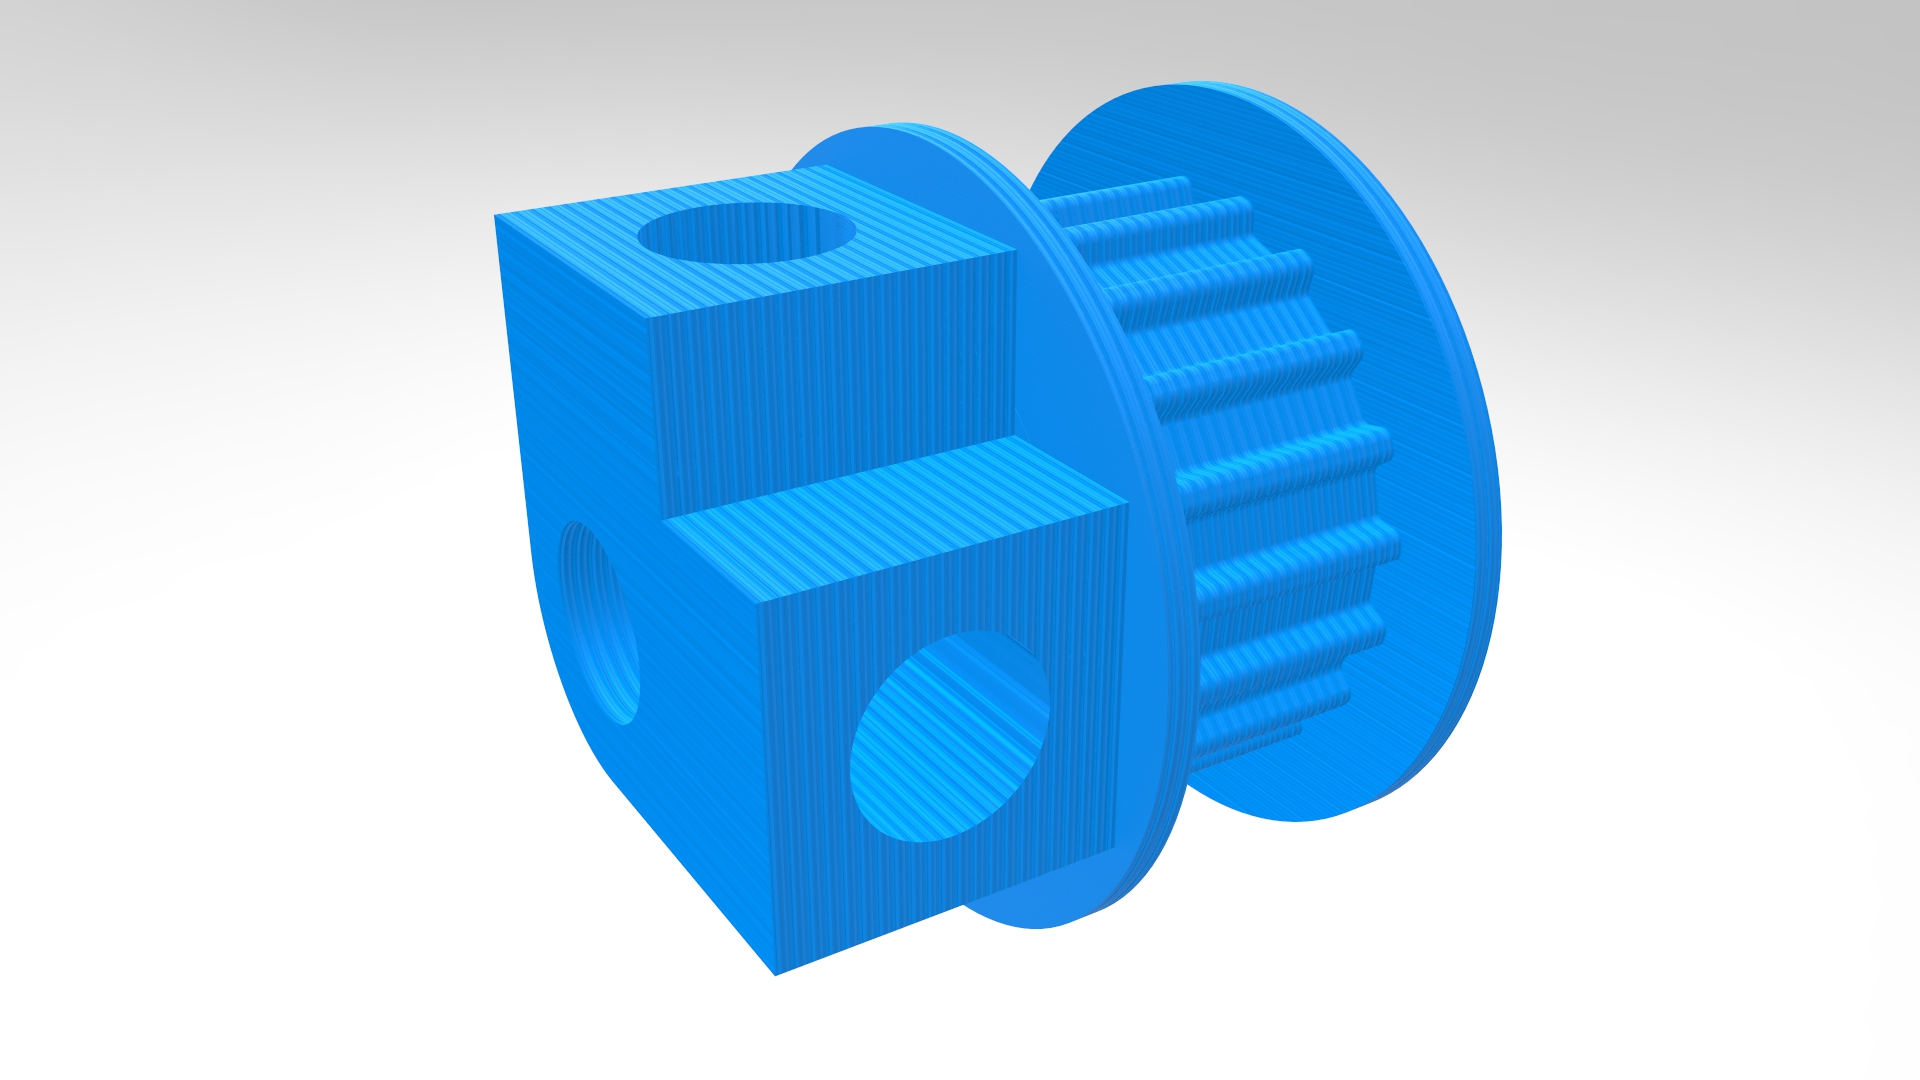
\includegraphics[width=\textwidth]{figures/legs_pulley_motor.jpg}
        \caption{Motor pulley}
        \label{fig:motor_pulley}
    \end{subfigure}
    \begin{subfigure}[b]{0.49\textwidth}
        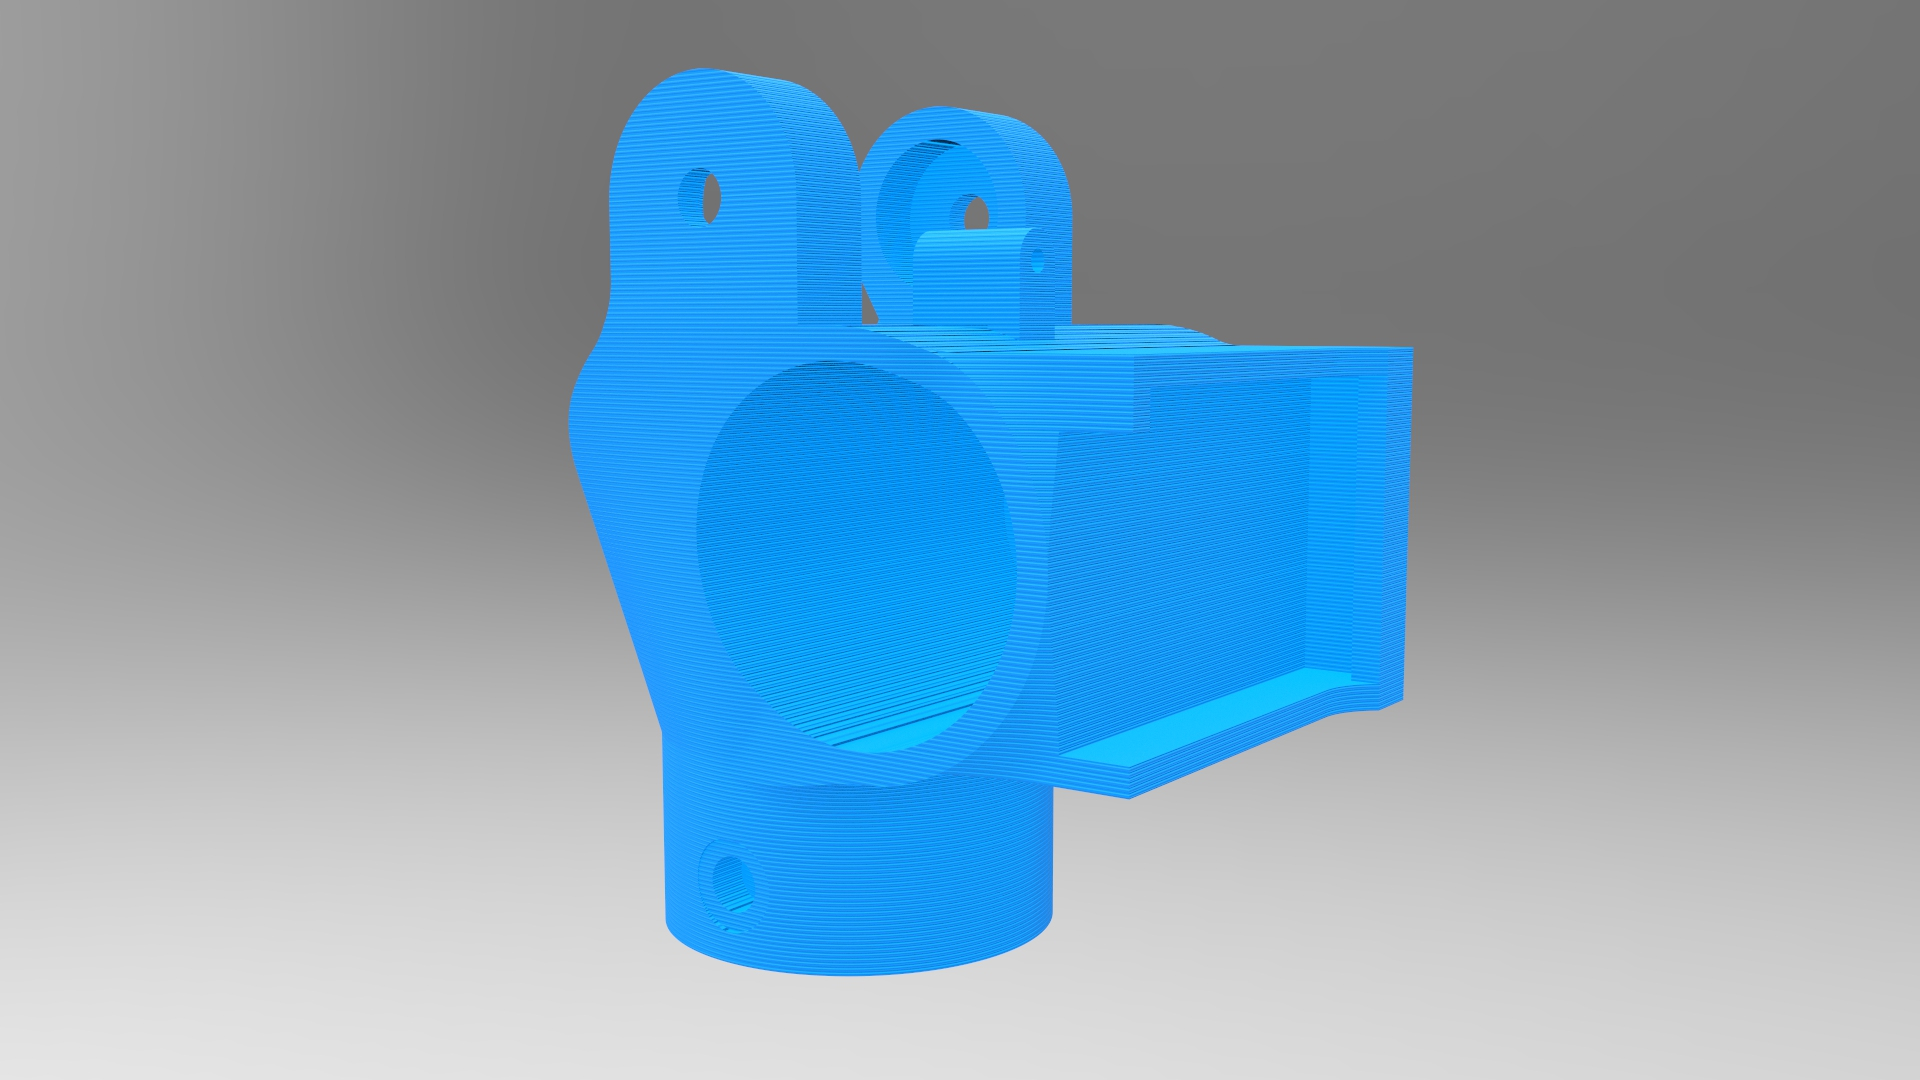
\includegraphics[width=\textwidth]{figures/legs_knee_lower.jpg}
        \caption{Left lower knee}
        \label{fig:lower_knee}
    \end{subfigure}
\end{figure}

\begin{figure}[ht!]
    \ContinuedFloat % continue from previous page
    \begin{subfigure}[b]{0.49\textwidth}
        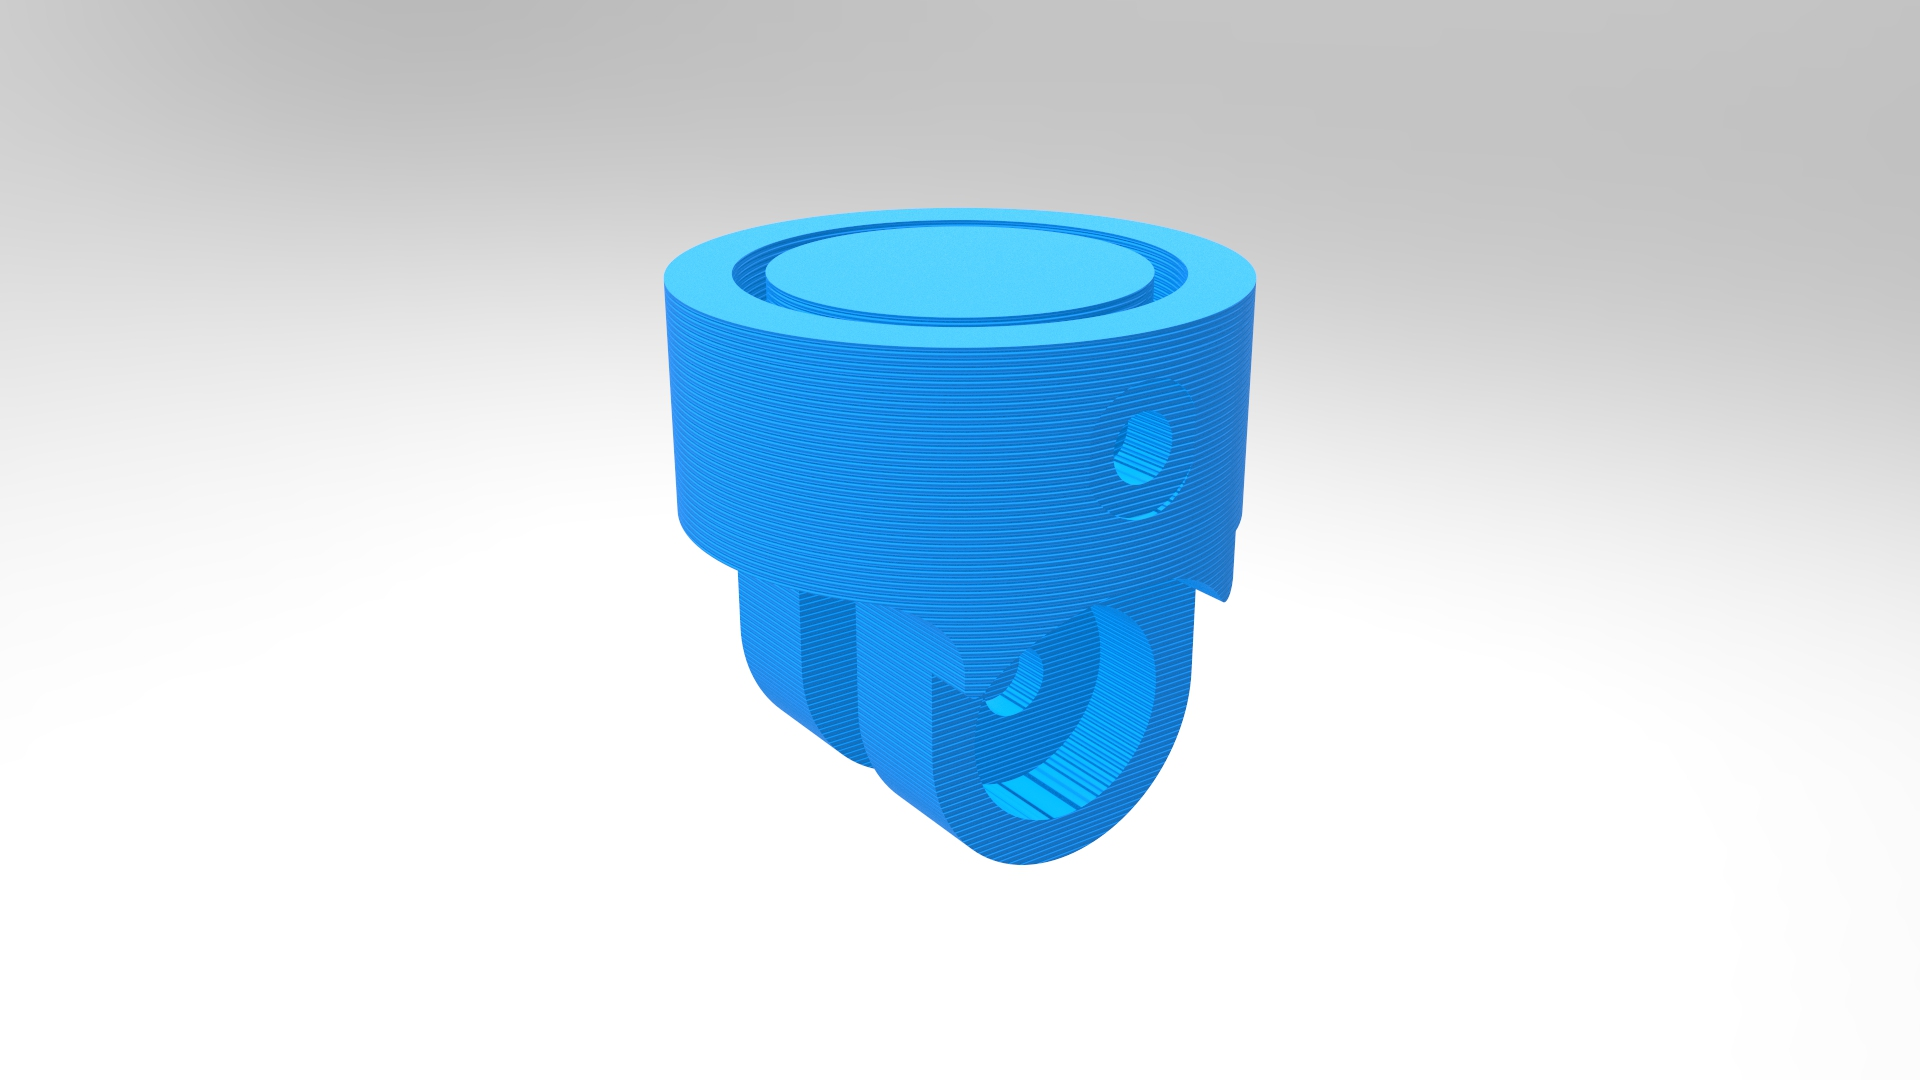
\includegraphics[width=\textwidth]{figures/legs_ankle_upper.jpg}
        \caption{Left upper ankle}
        \label{fig:ankle_upper}
    \end{subfigure}
    \begin{subfigure}[b]{0.49\textwidth}
        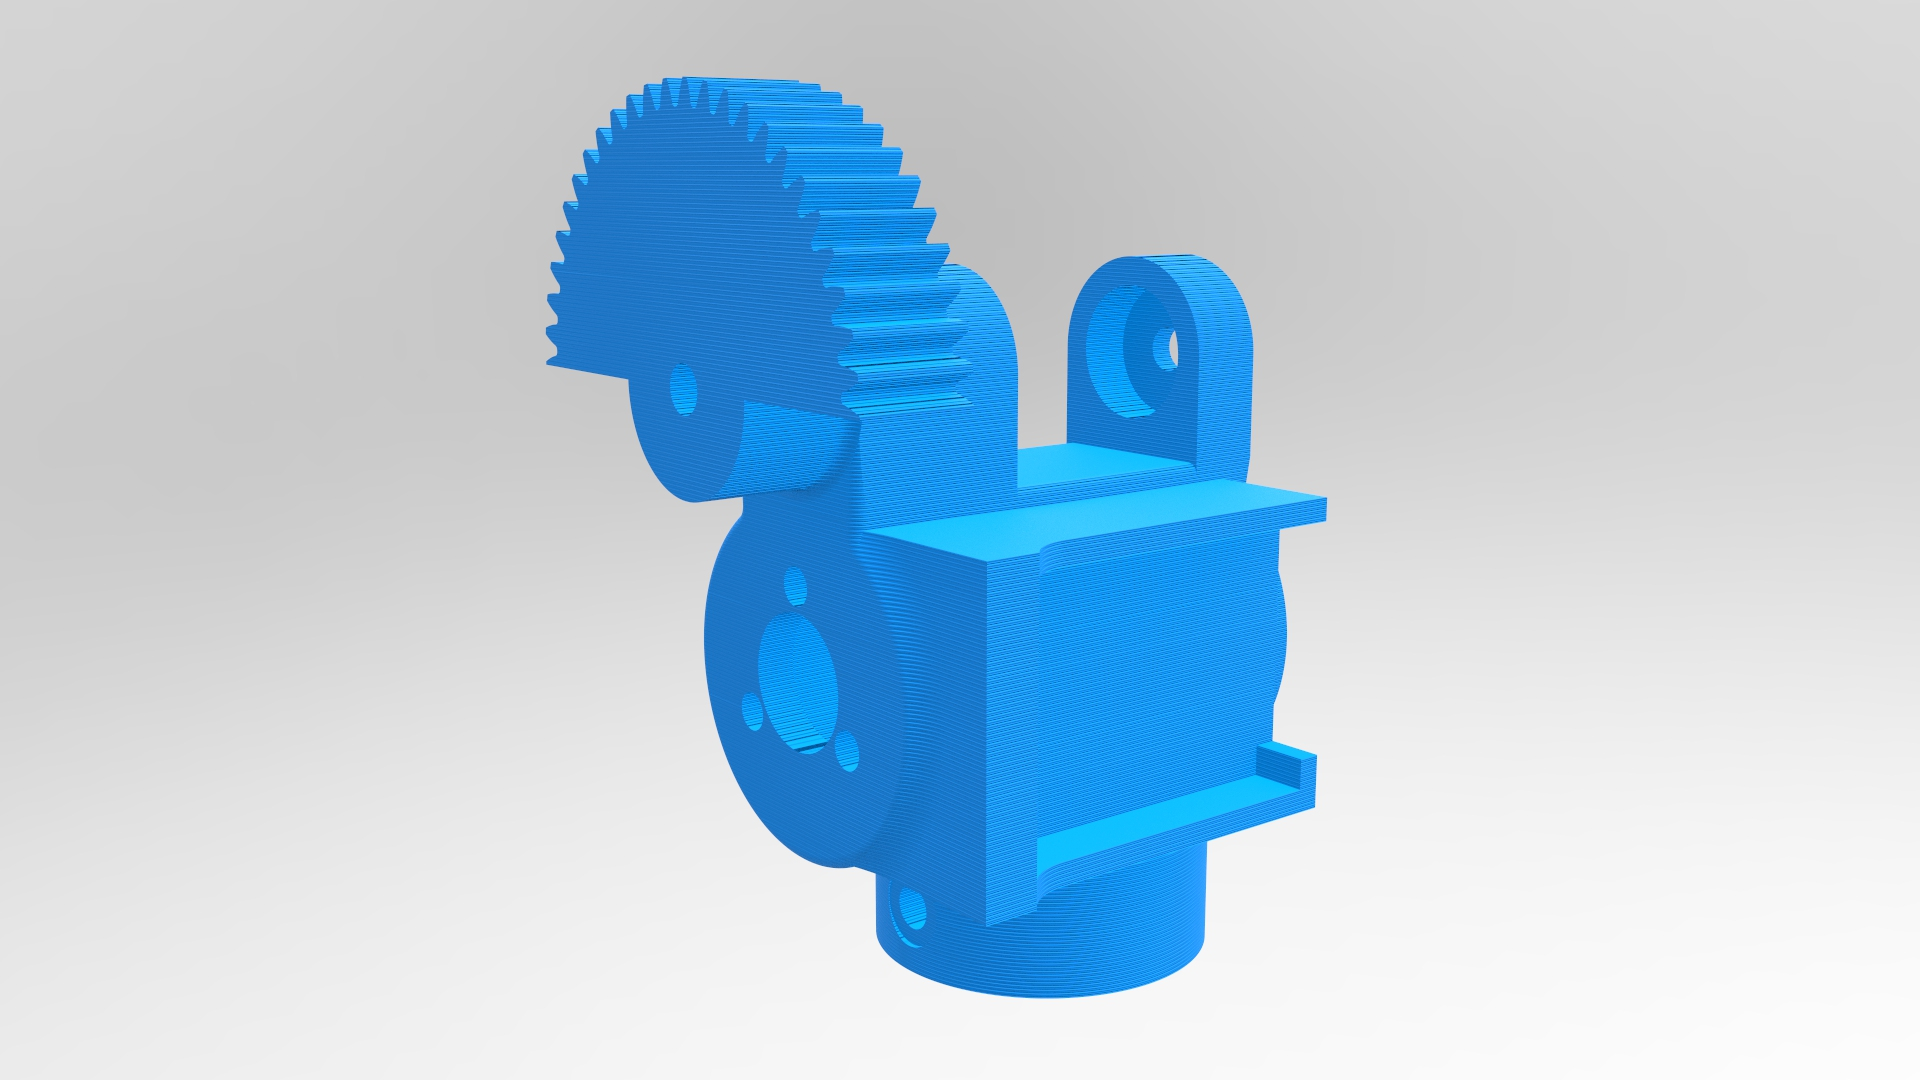
\includegraphics[width=\textwidth]{figures/legs_hip_lower.jpg}
        \caption{Left lower hip}
        \label{fig:hip_lower}
    \end{subfigure}
\end{figure}

\begin{figure}[ht!]
    \ContinuedFloat % continue from previous page
    \begin{subfigure}[b]{0.49\textwidth}
        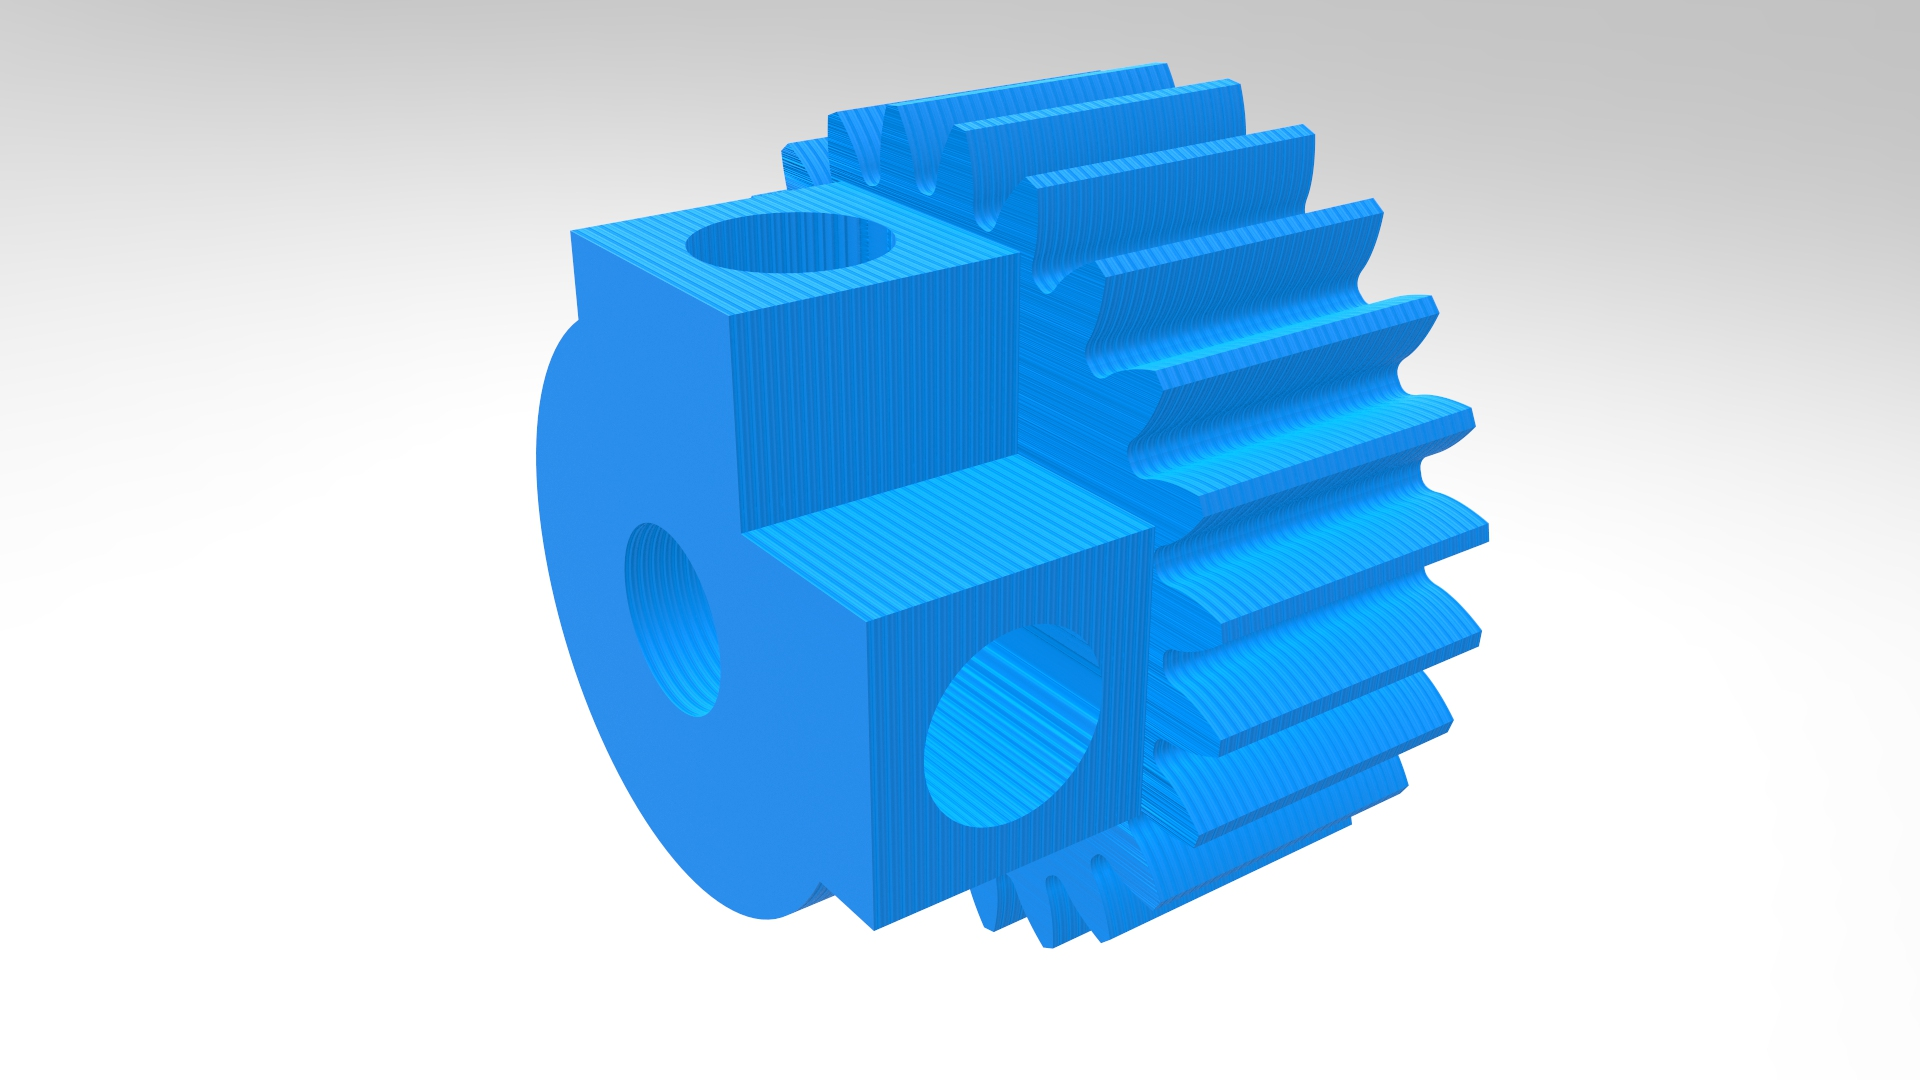
\includegraphics[width=\textwidth]{figures/legs_hip_pinion.jpg}
        \caption{Hip's pinion}
        \label{fig:hip_pinion}
    \end{subfigure}
    \begin{subfigure}[b]{0.49\textwidth}
        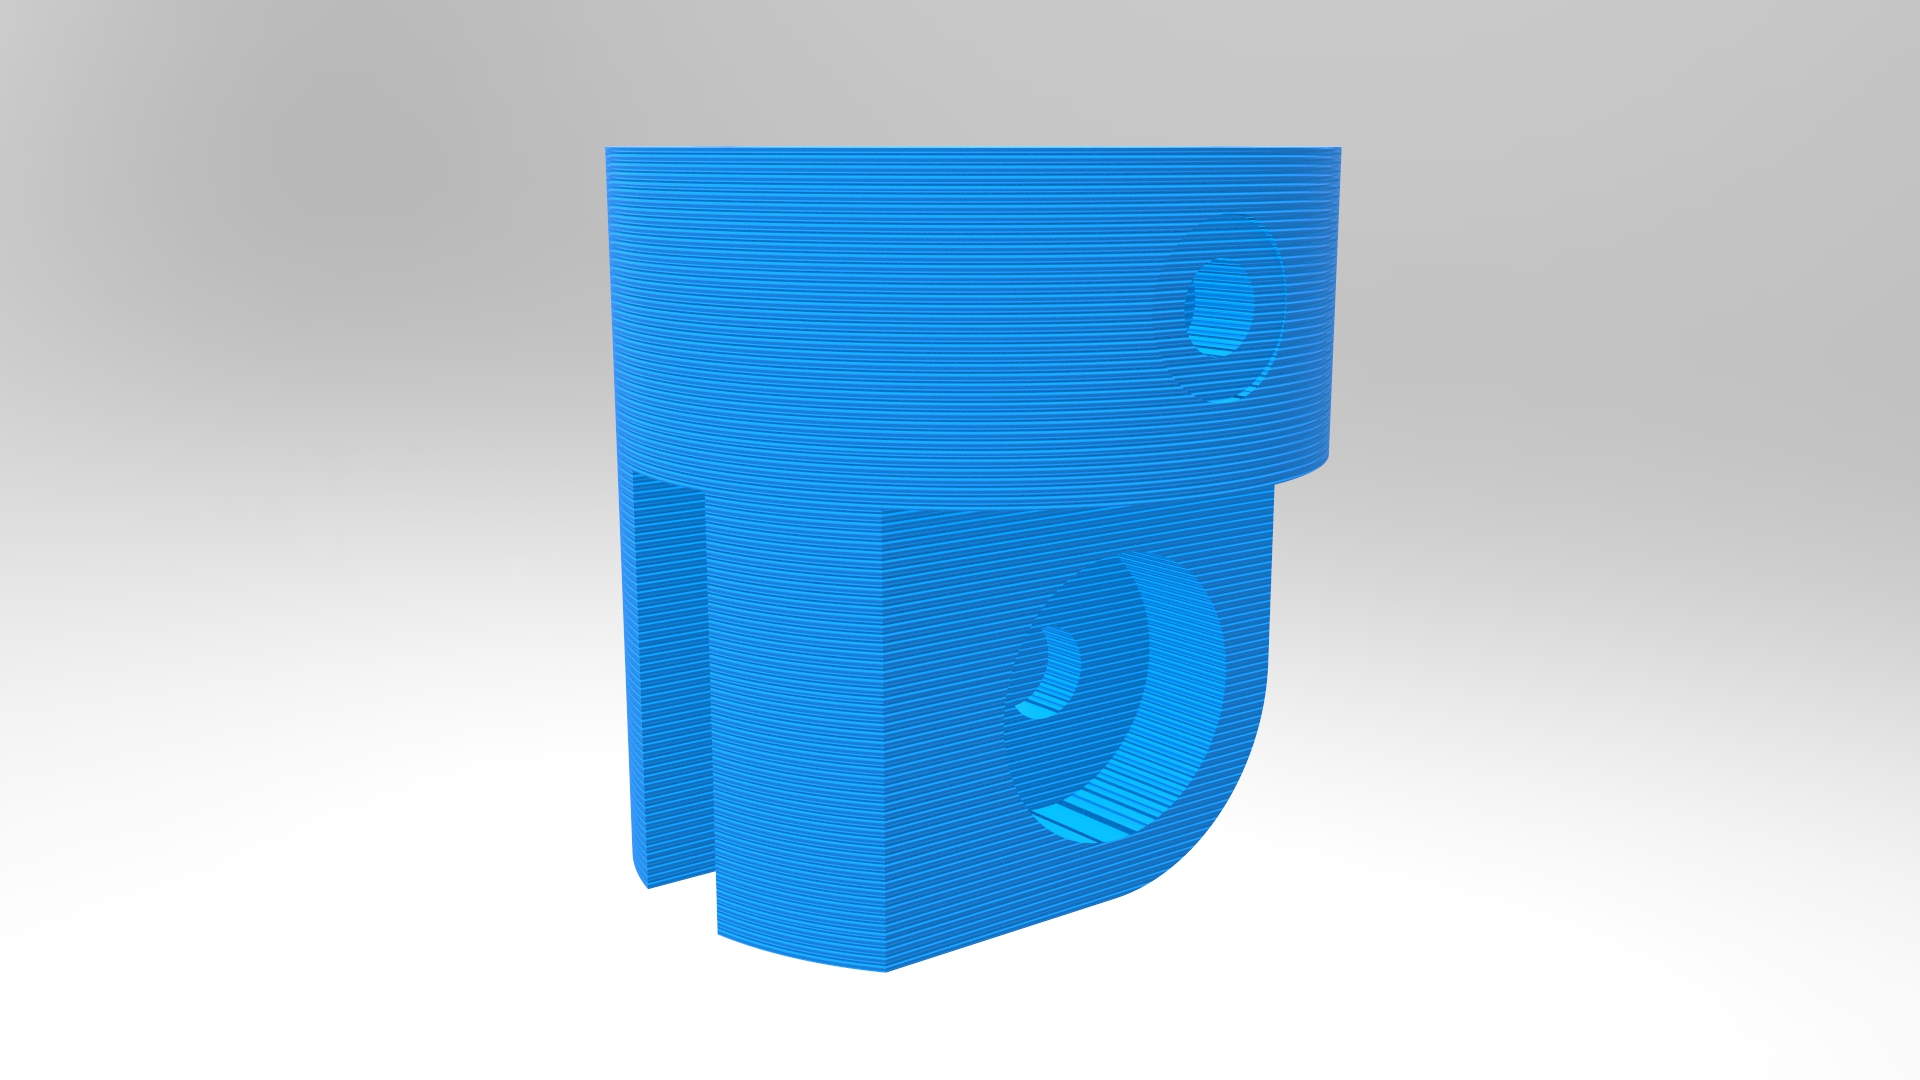
\includegraphics[width=\textwidth]{figures/legs_knee_upper.jpg}
        \caption{Left upper knee}
        \label{fig:knee_upper}
    \end{subfigure}
    \caption{Main CAD designed components}
\end{figure}

The CAD program has the feature of, given the physical properties of the materials or selecting one of the predefined, calculate the physical values such moments of inertia or center of gravity.
This has been used in the mathematical model \ref{cha:mathematical_model} to size the motors and in the simulation \ref{cha:simulation} to create the model as close to reality as possible.
The tables from \ref{tab:foot_physical_properties} to \ref{tab:total_mass} show the moments of inertia and total mass calculated by the CAD program.
The moments of inertia are taken from the appropriate rotation axis of the link.

\begin{table}[htbp]
\caption{Physical properties of the foot obtained from CAD program}
\begin{center}
\begin{tabular}{c|l|l}
\multicolumn{ 3}{c}{\Large \textbf{Foot}} \\
\multicolumn{ 3}{c}{\textbf{Mass $[Kg]$}} \\ \hline
\multicolumn{ 3}{c}{0.021} \\ \hline
\multicolumn{ 3}{c}{\textbf{Moments of inertia [$Kg \cdot m^2$] (Taken at output coordinate system)}} \\ \hline
Ixx = 2.2e-005 & \multicolumn{1}{c|}{Ixy = -9.16e-006} & \multicolumn{1}{c}{Ixz = 0} \\ \hline
Iyx = -9.16e-006 & \multicolumn{1}{c|}{Iyy = 9.05e-006} & \multicolumn{1}{c}{Iyz = 0} \\ \hline
Izx = 0 & \multicolumn{1}{c|}{Izy = 0} & \multicolumn{1}{c}{Izz = 2.88e-005} \\ 
\end{tabular}
\end{center}
\label{tab:foot_physical_properties}
\end{table}


\begin{table}[htbp]
\caption{Physical properties of the lower limb obtained from CAD program}
\begin{center}
\begin{tabular}{c|l|l}
\multicolumn{ 3}{c}{\Large \textbf{Lower limb}} \\
\multicolumn{ 3}{c}{\textbf{Mass $[Kg]$}} \\ \hline
\multicolumn{ 3}{c}{0.115} \\ \hline
\multicolumn{ 3}{c}{\textbf{Moments of inertia [$Kg \cdot m^2$] (Taken at the output coordinate system)}} \\ \hline
Ixx = 0.000699 & \multicolumn{1}{c|}{Ixy = 2.44e-005} & \multicolumn{1}{c}{Ixz = 0} \\ \hline
Iyx = 2.44e-005 & \multicolumn{1}{c|}{Iyy = 1.85e-005} & \multicolumn{1}{c}{Iyz = -1.82e-005} \\ \hline
Izx = 0 & \multicolumn{1}{c|}{Izy = -1.82e-005} & \multicolumn{1}{c}{Izz = 0.000694} \\ 
\end{tabular}
\end{center}
\label{tab:lower_limb_physical_properties}
\end{table}


\begin{table}[htbp]
\caption{Physical properties of the upper limb obtained from CAD program}
\begin{center}
\begin{tabular}{c|l|l}
\multicolumn{ 3}{c}{\Large \textbf{Upper limb}} \\
\multicolumn{ 3}{c}{\textbf{Mass $[Kg]$}} \\ \hline
\multicolumn{ 3}{c}{0.123} \\ \hline
\multicolumn{ 3}{c}{\textbf{Moments of inertia [$Kg \cdot m^2$] (Taken at the output coordinate system)}} \\ \hline
Ixx = 0.00119 & \multicolumn{1}{c|}{Ixy = 2.89e-006} & \multicolumn{1}{c}{Ixz = -1.36e-008} \\ \hline
Iyx = 2.89e-006 & \multicolumn{1}{c|}{Iyy = 1.69e-005} & \multicolumn{1}{c}{Iyz = -1.78e-005} \\ \hline
Izx = -1.36e-008 & \multicolumn{1}{c|}{Izy = -1.78e-005} & \multicolumn{1}{c}{Izz = 0.00118} \\ 
\end{tabular}
\end{center}
\label{tab:upper_limb_physical_properties}
\end{table}


\begin{table}[htbp]
\caption{Physical properties of the hip obtained from CAD program}
\begin{center}
\begin{tabular}{c|l|l}
\multicolumn{ 3}{c}{\Large \textbf{Hip}} \\ 
\multicolumn{ 3}{c}{\textbf{Mass $[Kg]$}} \\ \hline
\multicolumn{ 3}{c}{0.156} \\ \hline
\multicolumn{ 3}{c}{\textbf{Moments of inertia [$Kg \cdot m^2$] (Taken at the output coordinate system)}} \\ \hline
Ixx = 0.000303 & \multicolumn{1}{c|}{Ixy = 0} & \multicolumn{1}{c}{Ixz = 1.44e-008} \\ \hline
Iyx = 0 & \multicolumn{1}{c|}{Iyy = 2.78e-005} & \multicolumn{1}{c}{Iyz = 0} \\ \hline
Izx = 1.44e-008 & \multicolumn{1}{c|}{Izy = 0} & \multicolumn{1}{c}{Izz = 0.000314} \\ 
\end{tabular}
\end{center}
\label{tab:hip_physical_properties}
\end{table}


\begin{table}[htbp]
\caption{Total mass obtained from CAD program}
\begin{center}
\begin{tabular}{c|l|l}
\multicolumn{ 3}{c}{\Large \textbf{Total}} \\ 
\multicolumn{ 3}{c}{\textbf{Mass $[Kg]$}} \\ \hline
\multicolumn{ 3}{c}{0.707} \\ \hline
\end{tabular}
\end{center}
\label{tab:total_mass}
\end{table}


% subsection computer_aided_design (end)